\chapter{基于单张自然环境照片的人脸重建}
\label{chap:recon}

本章介绍了一种非常通用的人脸重建任务的实现,它能够从单张自然环境照片中重建人脸的3D模型。
自然环境照片指的是在室外或室内的自然光照条件下,使用手机等非专业设备拍摄的照片。
这类照片的中背景和环境光照通常都比较复杂,且受限于拍摄条件难以显式建模或捕获。
该实现输出的模型可以支持小范围的视角和光照变化,并可用于人脸编辑、人脸表情迁移、语音驱动等下游任务。

现有方法或者使用多帧、多视角监督,或者借助分割结果或人脸2D关键点检测结果辅助监督。
这些方法或对数据要求高,或有较严重的传递误差,或需要额外的人工标注。
本文则只是用单张照片,通过主要通过可微分渲染的监督信号完成重建,并集成现有神经网络和3DMM人脸模型提供正则化以提升优化的鲁棒性。
与关键点相比,可微分渲染方法能利用照片中的每一个像素,实现更加稠密的监督,从而理论上提升重建的精度。
然后,为了重现高分辨率的输入图像中的更多细节,本文使用了一些传统算法以生成高分辨率的纹理贴图。

\section{总体流程}

\begin{figure}
    \centering
    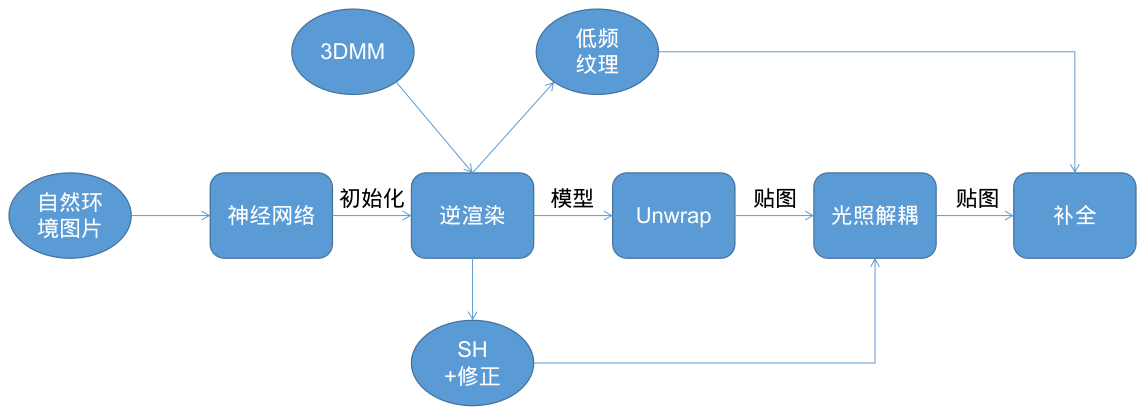
\includegraphics[width=0.95\linewidth]{figures/recon_overall}
    \caption{人脸重建总体流程}
    \label{fig:recon_overall}
\end{figure}

为完成该人脸重建的目标,本方法将输出一个基于预定义的拓扑结构的三角形网格,以及其对应的高清纹理贴图,该图的颜色表征人脸表面的光线反射率。
其总体流程如\ref{fig:recon_overall}所示。
本文首先利用现有方法\citep{deep3d}根据输入的照片估计3DMM人脸模型的形变系数,环境光照,人脸姿态等信息。
以此作为初始化,本文利用第\ref{chap:method}章提出的方法进一步将模型精确对齐到输入照片中,并进一步优化对环境光照的估计。
然后本文将照片的像素投影到纹理空间,依据估计的环境光照将照片中的光照效果和人脸本身的反射率分离,以支持渲染时的光照变化。
最后,本文利用3DMM建模的低频纹理对模型在照片中被遮挡的部分进行补全,以支持渲染时视角的变化。

后文将对该流程中的每个步骤进行详细介绍。

\section{基于神经网络回归的模型初始化}
\label{sec:recon_init}

基于可微分渲染的逆渲染方法通常难以处理较大的姿态变化,它容易在复杂的非线性优化中陷入局部最优。
因而之前很多方法均使用了2D人脸关键点检测结果以提供大范围的,较为平滑的监督信号。
然而关键的的位置定义是较为模糊的,3D模型上的标注和2D检测的误差都会导致误差传递到之后的步骤中。
而本文则不使用关键点以避免这些传递误差,同时免去模棱两可的3D模型关键点标注工作。
本文提出利用现有神经网络方法\citep{deep3d}通过输入照片估计其中人脸3DMM模型的形变系数,环境光照,人脸姿态等信息,并以此作为下一步骤的初始化。

\paragraph{人脸检测}
具体来说,对于一张输入的照片$\mathcal{I}\in\mathbb{R}^{H\times W\times 3}$,本文首先在其中检测人脸。
在输入前本文首先对照片$\mathcal{I}$进行$N$倍降采样(平均池化)为$\mathcal{I}_m$以控制检测的资源消耗,其中$N=\left\lceil \max(H, W) / 1024\right\rceil$,也就是将最长边控制在1024像素以内。
本文使用了\citet{SFD}开源的人脸检测软件。
该软件能输出矩形人脸检测框,本文选择其输出的面积最大的检测框$B$。

\paragraph{系数预测}
然后本文进一步将照片$\mathcal{I}_m$降采样为$\mathcal{I}_s\in\mathbb{R}^{224\times 224\times 3}$,将检测框包含在其中并使其面积最大且居中。
若裁剪框超出像素边缘则填充黑色,以保持人脸在图像中心。
然后$\mathcal{I}_s$将输入到\citet{deep3d}开源的软件中,
它将输出BFM模型\citep{BFM}的
人脸身份系数$\mathbf{\alpha}\in\mathbb{R}^{80}$,
人脸表情系数$\mathbf{\beta}\in\mathbb{R}^{64}$,
人脸纹理系数$\mathbf{\delta}\in\mathbb{R}^{80}$,
人脸姿态$\mathbf{p}\in\mathrm{SE(3)}$,
环境球谐光照系数$\mathbf{\gamma}\in\mathbb{R}^{9\times 3}$。
其中涉及到的3D坐标均可通过约定的投影矩阵$\mathbf{P}_\mathrm{d}$投影回图像平面,并与输入图像$\mathcal{I}_s$较好地对齐。

\paragraph{坐标系转换}
然而,上一步骤预测时使用的投影矩阵是固定的,而输入的照片拍摄时使用的设备,人脸在照片中的尺寸,位置都有不同。
为了获取尽可能精确的结果,本文试图从照片的元数据中提取相机实际参数,结合裁减的方式,计算更准确的投影矩阵,并将所涉及到的3D坐标在不同投影矩阵间进行转换,同时满足:3D点在图像上投影的位置基本不变;人脸模型在3D空间的尺度基本不变。

此处投影矩阵定义为$3\times 3$的矩阵$\mathbf{P}$,其使用方式为$\mathbf{x} = \mathbf{P}\mathbf{X}$,
其中$\mathbf{X}$为相机坐标系下的点的三维坐标,$(\mathbf{x}_x/\mathbf{x}_z,\mathbf{x}_y/\mathbf{x}_z)\in[-1,1]^2$即是该点投影到图像上的二维坐标。
注意此处的图像坐标系与图像分辨率无关,这与OpenGL等渲染库的约定一致,且便于后续在不同投影矩阵转换时的计算。
但与OpenGL中常用的投影矩阵形式不同,为了简化推导,此处的投影矩阵并未投影深度。
可从照片的EXIF中提取的信息包括相机焦距$f\in\mathbb{R}$,分辨率$\mathbf{r}\in\mathbb{R}^2$,传感器像素密度$\mathbf{\rho}\in\mathbb{R}^2$。
根据这些信息,并假设该相机符合完美的小孔成像模型,则该相机的投影矩阵为:
\begin{equation}
    \mathbf{P}_\mathrm{cam} = \begin{bmatrix}
        \frac{2f\mathbf{\rho}_x}{\mathbf{r}_x} & 0 & 0 \\
        0 & \frac{2f\mathbf{\rho}_y}{\mathbf{r}_x} & 0 \\
        0 & 0 & 1
    \end{bmatrix}
    \text{。}
\end{equation}
进一步地,裁减操作可以看作是平移和缩放操作的组合,记裁剪框的左下角和右上角坐标分别为$\mathbf{p}_\mathrm{min},\mathbf{p}_\mathrm{max}\in[-1,1]^2$,
则裁剪框内区域的投影矩阵为:
\begin{equation}
    \mathbf{P}_\mathrm{crop} = \begin{bmatrix}
        \frac{2}{\mathbf{p}_\mathrm{max,x}-\mathbf{p}_\mathrm{min,x}} & 0 & 0 \\
        0 & \frac{2}{\mathbf{p}_\mathrm{max,y}-\mathbf{p}_\mathrm{min,y}} & 0 \\
        0 & 0 & 1
    \end{bmatrix}\begin{bmatrix}
        1 & 0 & -\frac{\mathbf{p}_\mathrm{min,x}+\mathbf{p}_\mathrm{max,x}}{2} \\
        0 & 1 & -\frac{\mathbf{p}_\mathrm{min,y}+\mathbf{p}_\mathrm{max,y}}{2} \\
        0 & 0 & 1
    \end{bmatrix}\mathbf{P}_\mathrm{cam}
    \text{。}
\end{equation}

以下将介绍具体如何将3D模型从投影矩阵$\mathbf{P}_\mathrm{d}$转换到$\mathbf{P}_\mathrm{crop}$下。
该转换分为两步,将模型关于相机旋转以保持模型中心点投影位置不变,再将模型向朝向或远离相机的方向平移以保持模型的投影尺度不变。
这两步操作均为刚性变换,因此可以保证模型在3D空间的尺度不变。

首先求解旋转,该步骤主要用于平衡不同照片中人脸裁剪框位置的差异。
记3D网格模型$M=\{\mathbf{v}_i\}_i$为三维顶点的集合,其中$\mathbf{v}_i\in\mathbb{R}^3$为神经网络预测的顶点的三维坐标。
记$\bar{\mathbf{v}} = \frac{1}{|M|}\sum_{i=1}^{|M|}\mathbf{v}_i$为模型中心点的三维坐标。
若要该中心点的投影位置不变,则该点应位于新坐标系下的一条以原点为起点的射线上,该射线上另一点的坐标为$\bar{\mathbf{v}}' = \mathbf{P}_\mathrm{crop}^{-1}\mathbf{P}_\mathrm{d}\bar{\mathbf{v}}$。
因此,所需旋转的旋转轴为$\bar{\mathbf{v}}' \times \bar{\mathbf{v}}$,
旋转角为$\arccos\left(\frac{\bar{\mathbf{v}}'\cdot\bar{\mathbf{v}}}{\|\bar{\mathbf{v}}'\|\|\bar{\mathbf{v}}\|}\right)$。
可由罗德里格斯公式计算其对应旋转矩阵$\mathbf{R}$,类似公式\ref{eq:rodrigues},此处不再赘述。
旋转后的中心点坐标记为$\bar{\mathbf{v}}'' = \mathbf{R}\bar{\mathbf{v}}$。

然后可以求解所需平移,该步骤主要用于平衡不同相机的焦距参数的差异。
记平移后的中心点位置为$\bar{\tilde{\mathbf{v}}} = s\bar{\mathbf{v}}''$,
$s$表示平移前后该点据相机的距离比例。
若要模型投影尺度不变,则$s$应满足如下方程:对于三维坐标$\mathbf{x}=[x,y,z]^\mathsf{T}$
\begin{equation}
    \left.\nabla_{x,y}\left(\frac{\mathbf{P}_\mathrm{crop}\mathbf{x}}{z}\right)\right|_{\mathbf{x}=\bar{\tilde{\mathbf{v}}}} =
    \left.\nabla_{x,y}\left(\frac{\mathbf{P}_\mathrm{d}\mathbf{x}}{z}\right)\right|_{\mathbf{x}=\bar{\mathbf{v}}}
    \text{。}
\end{equation}
该方程是超定方程,但由于这里使用的投影矩阵均是按相同比例处理x和y轴的,因此应当能解出一致的$s$。在实践中可以使用最小二乘法求解。

在得到针对模型中心点的变换参数后,将这些变换应用到整个模型即可完成坐标系的转换。
转换后的顶点坐标为:
\begin{equation}
    \tilde{\mathbf{v}}_i = \mathbf{R}\mathbf{v}_i + \left( \bar{\tilde{\mathbf{v}}} - \bar{\mathbf{v}}'' \right)
    \text{,}
\end{equation}
转换后的模型即为$\tilde{M}=\{\tilde{\mathbf{v}}_i\}_i$。
图\ref{fig:crop}用一个玩具实验展示了转换前后的模型,以及该转换的必要性。

\section{模型裁剪边缘的梯度处理}
\label{sec:recon_sdf}

可微分渲染在应用到人脸3D重建时有一个特殊的问题:人是一个很大的物体,而人脸重建的目标通常仅仅是人脸的这一小块区域。
所以通常在人脸重建中用于逆渲染的模型都是裁剪过的,只包含人脸的部分,因此具有一些人为制造的边缘。
这些边缘在照片中并不存在,但第\ref{chap:method}章提出的方法在应用到人脸时却也会在这些边缘产生相关梯度,由于并无对应的边缘可供对齐,这些梯度将导致模型过度扩展,影响最终收敛的效果。

解决该问题的关键在于如何判断渲染图像中的像素与模型指定边缘的位置关系,以便在计算梯度时能够区分人为制造的边缘和真正需要优化的边缘。
对此,本文受到\citet{sdf_glyphs}的启发,该作者提出使用SDF(Signed Distance Field,有向距离场)贴图来绘制可任意放大的矢量图形,并能根据SDF的梯度判断像素到图形边缘的距离,从而实现各向异性的抗锯齿。
于是,本文提出一种简单的基于SDF贴图的方法来区分人为制造的和真正需要优化的边缘。

具体地,本文定义一种SDF贴图。
对于该贴图中的每个像素,其值为一个单通道浮点数$d$,表示该像素点到最近的人为制造边缘的距离,在模型内部的为正,模型外部的为负,
如图\ref{fig:sdf}所示。
由于该贴图中并无太多高频信息,本文仅使用了$256 \times 256$的分辨率。
虽然似乎只有模型内部的贴图像素才会在渲染时被采样到,只需要计算模型内部的正值即可,但实际上,由于采样时使用双线性插值,外部的负值也会被采样到从而参与插值计算中.
更准确的线性插值结果正是SDF的主要优势之一。
从图中也可见,无论是SDF值还是其梯度在穿过边缘时都依然是平滑的。

\begin{figure}
\centering
\begin{subfigure}[t]{3.3in}
    \centering
    \import{build/figures}{sdf.pgf}
    \caption{SDF贴图}
    \label{fig:sdf}
\end{subfigure}
\begin{subfigure}[t]{2.9in}
    \centering
    \import{build/figures}{sdf_grad.pgf}
    \caption{SDF的梯度}
    \label{fig:sdf_grad}
\end{subfigure}
\caption[SDF贴图可视化]{SDF贴图可视化。灰色线为模型中人为制造的边缘。(a)为SDF贴图,表示每个像素到最近边缘的距离,模型内部为正,外部为负;(b)为(a)的梯度向量,其x和y分量分别可视化为红色和绿色通道。}
\end{figure}

下面以nvdiffrast的工作方式为例说明该贴图的使用方式:
nvdiffrast抗锯齿模块工作时将以一对相邻的像素点为单位(如图\ref{fig:aa}),其中一个像素在模型内部,另一个像素在模型外部。
对于处于模型内部的像素,可从SDF贴图中采样其对应的$d$值,并计算$\frac{\partial d}{\partial \mathbf{x}}$,其中$\mathbf{x}$为对应外部像素相对该内部像素的坐标偏移量。
也即对3D模型的表面在该内部像素点的位置使用一个平面进行一阶近似,并求外部像素在该近似平面上的位置,以估计外部像素是否在人为制造边缘之外。
正式地,对于一对分别处于模型内外的像素点,其处于人为制造的边缘当且仅当:
\begin{equation}
    d + \max\left(a\frac{\partial d}{\partial \mathbf{x}}, \delta\right) < 0
    \text{,}
\end{equation}
此时应该忽略其产生的可见性梯度。其中$\delta=0.1$为人为限制的梯度的最大值,为避免小概率时过大梯度产生过于离谱的结果;$a=1.5$为梯度放大的系数,为避免偶发的由于精度不足导致的检测遗漏。
这两个超参数的选择对最终结果的影响不大。

\begin{figure}
\centering
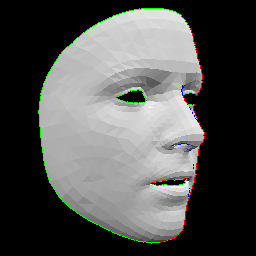
\includegraphics[height=2.2in]{figures/debug_sdf}
\caption[人为制造边缘分类效果]{人为制造边缘分类效果。绿色为人为制造的边缘;红色为与未知背景间的边缘;蓝色为模型内部相互遮挡产生的边缘。}
\label{fig:sdf_result}
\end{figure}

该算法对边缘分类的效果如图\ref{fig:sdf_result}所示。
可见算法将所有边缘分为了三类,
其中绿色为人为制造而需要忽略的边缘,
红色为与未知背景间的边缘,可按照第\ref{chap:method}章提出的方法进行处理,
蓝色为模型内部相互遮挡产生的边缘,应按正常可微分渲染流程处理。
从图中可见一些红色与绿色交错的区域,这是由于这两种边缘本身并没有明确的界限,有时人为制造的边界会正好投影到实际边界附近。
因此本文认为这种现象是十分合理且可接受的。

\paragraph{SDF贴图的计算}
关于SDF的计算方法有很多,下面介绍本文的实现方式。
本文首先使用Blender将3D人脸模型展开至纹理空间,然后在展开后的所有三角形中查找仅属于一个三角形的边做为所谓人为制造的边缘。
并将这些边加入CGAL封装的层次包围盒\footnote{https://doc.cgal.org/latest/AABB\_tree/index.html}数据结构中,以便快速查找。
随后调用OpenGL将所有展开后的三角形光栅化渲染至图像中,得到边缘内部像素的遮罩。
最后,对于贴图中的每个像素,从层次包围盒中查找与其最近的边,计算其与该边的距离$|d|$,并根据遮罩赋予其符号。$d$的梯度方向即为从该像素指向该边上与其最近点的方向(或反方向),模长为$1$。
本方法相比\citet{sdf_glyphs}介绍的暴力方法效率更高,本方法计算$256\times256$分辨率的贴图,使用CPU单线程用时在10毫秒左右。

\paragraph{梯度计算}
梯度$\frac{\partial d}{\partial \mathbf{x}}$的计算与所使用的渲染方式有关。
例如OpenGL支持通过数值方法直接求任意变量关于像素坐标的梯度\footnote{https://registry.khronos.org/OpenGL-Refpages/gl4/html/dFdx.xhtml}。
而针对本文使用的nvdiffrast来说,本文首先以解析法随SDF一同计算其关于纹理坐标的梯度$\frac{\partial d}{\partial u}$和$\frac{\partial d}{\partial v}$,并将其与$d$一同保存于贴图中。
然后根据nvdiffrast的插值模块给出的纹理坐标和像素坐标间的雅可比矩阵将其到像素坐标:
\begin{equation}
    \begin{bmatrix}
        \frac{\partial d}{\partial x} \\
        \frac{\partial d}{\partial y}
    \end{bmatrix} = \begin{bmatrix}
        \frac{\partial u}{\partial x} & \frac{\partial u}{\partial y} \\
        \frac{\partial v}{\partial x} & \frac{\partial v}{\partial y}
    \end{bmatrix} \begin{bmatrix}
        \frac{\partial d}{\partial u} \\
        \frac{\partial d}{\partial v}
    \end{bmatrix}
\text{。}
\end{equation}
该方法与\citet{sdf_glyphs}中提出的方法相同。
所要求的$\frac{\partial d}{\partial \mathbf{x}}$根据前景和背景像素的相对位置,是$\frac{\partial d}{\partial x}$或$\frac{\partial d}{\partial y}$或其相反数四者之一。

另一种解决该问题的可能的方案是屏蔽位于模型表面特定区域的像素上的可见性梯度,例如屏蔽特定三角形,屏蔽到边缘距离小于某个阈值的区域,手动指定遮罩等。
相比于这些方法,本方法具有如下优势:
\begin{enumerate}
\item 渲染尺度无关:同样的模型区域在不同尺度下渲染呈现的尺度不同,因此屏蔽区域的选择可能需要随着尺度变化而改变。
而本方法融入$d$了对像素坐标的梯度信息,是模型表面的一阶近似,因此不受尺度的影响。
\item 有向性:即使是同一个像素,在其不同方向上也可能分别靠近不同种类的边缘。
本方法通过考虑$d$的梯度方向,可以区分这些不同的边缘。
\end{enumerate}

\section{基于可微分渲染的逆渲染优化}

\begin{figure}
\centering
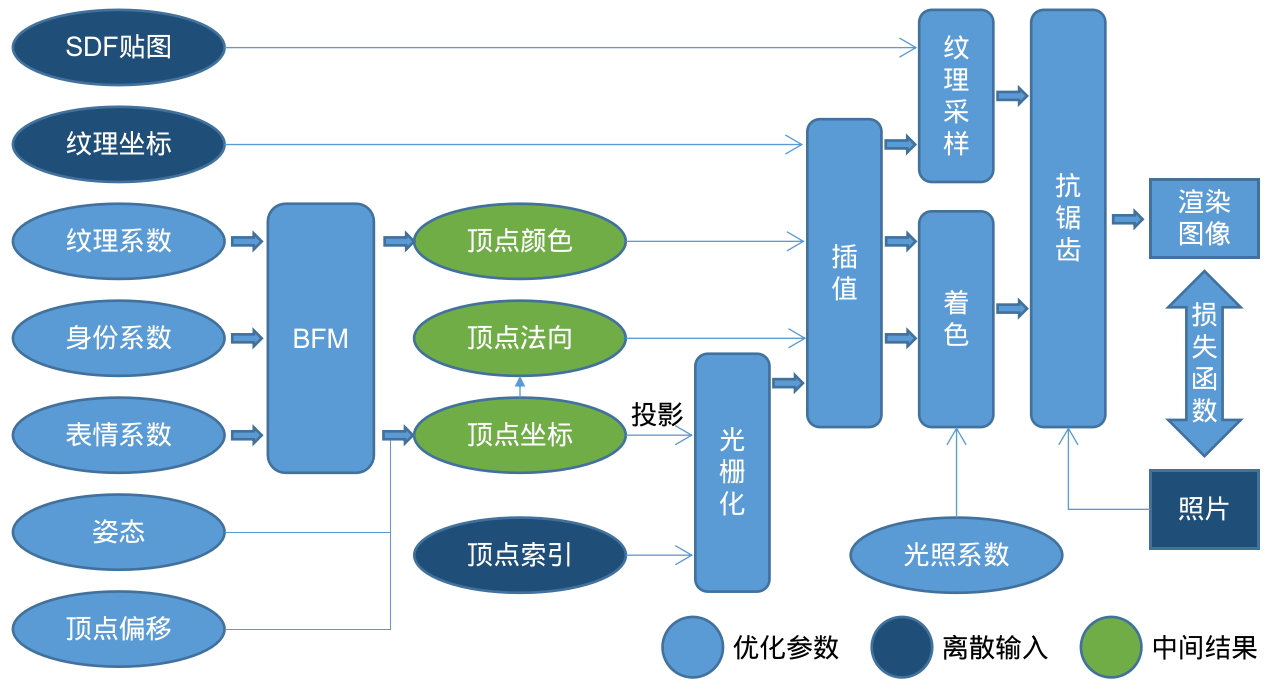
\includegraphics[width=\linewidth]{figures/recon_render}
\caption{渲染的整体流程}
\label{fig:recon_render}
\end{figure}

基于第\ref{sec:recon_init}节计算的3D模型、纹理、环境光照估计作为初始化,
以及第\ref{chap:method}章和第\ref{sec:recon_sdf}节提出的方法,
本节具体将介绍如何将它们结合nvdiffrast\citep{nvdiffrast}实际应用于人脸3D模型的逆渲染过程中。
渲染的整体流程如图\ref{fig:recon_render}所示。
逆渲染的目标即是通过梯度下降优化的方式,优化模型参数,使得渲染结果与照片尽可能接近。
以下将具体介绍该流程中的各个步骤。

\paragraph{顶点计算和投影}
首先本文实现了类似传统渲染引擎中的顶点着色器的计算。
这个步骤输入模型的各种数据和参数,输出该模型每个顶点在裁切空间中的坐标,以及定义在每个顶点上的一些附加属性。
本文由是使用的着色模型较为简单,因此附加属性仅包括法线,颜色和纹理坐标。

首先,本文依据类似3DMM模型的方式计算其每个顶点的位置和颜色:
\begin{align}
\mathbf{S} &= \bar{\mathbf{S}} + \mathbf{B}_\mathrm{id}\mathbf{\alpha} + \mathbf{B}_\mathrm{exp}\mathbf{\beta} + \mathbf{S}_\mathrm{off}\\
\mathbf{T} &= \bar{\mathbf{T}} + \mathbf{B}_\mathrm{tex}\mathbf{\delta}
\text{。}
\end{align}
其中$\bar{\mathbf{S}}$和$\bar{\mathbf{T}}$分别是平均的人脸形状和纹理,
$\mathbf{B}_\mathrm{id}$、$\mathbf{B}_\mathrm{exp}$和$\mathbf{B}_\mathrm{tex}$分别是身份、表情和纹理的PCA基,并预先根据其对应的标准差进行了放大。
与之前方法\citep{deep3d,GuoZCJZ19}保持一致,本文使用了BFM 2009模型\citep{BFM}中的身份和纹理基,以及Face Warehouse\citep{FaceWarehouse}中的表情基。
$\mathbf{\alpha}$、$\mathbf{\beta}$和$\mathbf{\delta}$分别是身份、表情和纹理的系数,是所需优化的参数。
与之前的方法不同,本文使用了\ref{sec:recon_init}节中预测的系数来计算$\bar{\mathbf{S}}$和$\bar{\mathbf{T}}$,从而利用神经网络中的知识作为逆渲染优化的先验。
此外,本文还额外对顶点位置增加了一个偏移量$\mathbf{S}_\mathrm{off}$,以允许其偏离PCA产生的低维空间,拟合更加多样的人脸形状,从而充分发挥逆渲染用于监督的信息量大的优势。

在获得顶点位置后,还需将其变换到相机坐标系并投影到裁切空间中,以便后续的光栅化。投影后顶点在裁切空间中的坐标为:
\begin{equation}
\mathbf{S}_\mathrm{clip} = \mathbf{P}_\mathrm{crop}\mathbf{M}_\mathrm{c}\mathbf{M}_\mathrm{t}\mathbf{M}_\mathrm{d}\mathbf{S}
\text{,}
\end{equation}
其中$\mathbf{M}_\mathrm{c}\in \mathrm{SE(3)}$是可优化的参数。
该步骤在之前第\ref{sec:recon_init}节神经网络预测和坐标系转换后的结果的基础上,再增加了一个参数以供逆渲染过程进一步优化。
\TODO{更新前面的定义}


除了顶点位置和颜色,本文还计算了每个顶点的法线。
通行的做法是根据顶点周围的三角形的形状,对三角形的发现做加权平均。
但由于BFM模型的网格较为密集且均匀,简单起见,本文直接使用了与每个顶点相邻的多个三角形的法线平均值作为该顶点的法线。即第$i$个顶点的法线为:
\begin{equation}
\mathbf{N}_i \propto \sum_{j\in\mathcal{N}_i}\mathbf{N}_{tri,j} \quad
\|\mathbf{N}_i\| = 1
\text{,}
\end{equation}
其中$\mathcal{N}_i$是与顶点$i$相邻的三角形的集合,$\mathbf{N}_{tri,j}$是三角形$j$的法线。
之所以不直接使用每个三角形的法线进行着色(即如图\ref{fig:sdf_result}中的着色效果),
是希望在图像中法线方向是平滑变化的,不会在三角形交界处出现明显的跳变。

\paragraph{光栅化}
该步骤直接使用了

\section{照片到纹理空间信息迁移}

\section{实验结果}

\section{局限性}
